% geometrical-ray-tracing: Program to perform geometrical ray tracing
% Copyright (C) 2022  Tom Spencer (tspencerprog@gmail.com)
%
% This file is part of geometrical-ray-tracing
%
% geometrical-ray-tracing is free software: you can redistribute it and/or modify
% it under the terms of the GNU General Public License as published by
% the Free Software Foundation, either version 3 of the License, or
% (at your option) any later version.
%
% This program is distributed in the hope that it will be useful,
% but WITHOUT ANY WARRANTY; without even the implied warranty of
% MERCHANTABILITY or FITNESS FOR A PARTICULAR PURPOSE.  See the
% GNU General Public License for more details.
%
% You should have received a copy of the GNU General Public License
% along with this program.  If not, see <https://www.gnu.org/licenses/>.


\documentclass{article}
\usepackage[utf8]{inputenc}
\usepackage[a4paper, total={6in, 8in}]{geometry}
\usepackage{amsmath}
\usepackage{bm}
\usepackage{datetime}
\usepackage{caption}
\usepackage{subcaption}
\usepackage{tikz}

\def\bibsection{\section*{References}} 

\usepackage{listings}  % For nicely displaying Python code
\usepackage{xcolor}
\definecolor{keywords}{RGB}{255,0,90}
\definecolor{comments}{RGB}{0,150,0}
\definecolor{black}{RGB}{0,0,0}
\definecolor{green}{RGB}{0,171,46}
\definecolor{purple}{RGB}{125,17,23}
\definecolor{orange}{RGB}{240,109,18}
\definecolor{blue}{RGB}{17,38,208}
\definecolor{red}{RGB}{191,3,20}

% Redefining vectors and define unit vectors
\let\vec \bm
\newcommand{\uveci}{{\bm{\hat{\textnormal{\bfseries\i}}}}}
\newcommand{\uvecj}{{\bm{\hat{\textnormal{\bfseries\j}}}}}
\DeclareRobustCommand{\uvec}[1]{{%
  \ifcsname uvec#1\endcsname
     \csname uvec#1\endcsname
   \else
    \bm{\hat{\mathbf{#1}}}%
   \fi
}}

% differential operator
\newcommand{\diff}{\textnormal{d}}

% remove math formatting
\newcommand{\mrm}[1]{\mathrm{#1}}


\title{geometrical-ray-tracing}
\author{Tom Spencer}
\date{\currenttime, \today}

\begin{document}

\lstset{language=Python, 
        basicstyle=\ttfamily\small, 
        morekeywords={self},
        keywordstyle=\color{orange},
        commentstyle=\color{red},
        stringstyle=\color{green},
        showstringspaces=false,
        identifierstyle=\color{black},
}

\maketitle

\section{Introduction}
\texttt{geometrical-ray-tracing} is a Python library that performs geometrical ray tracing in two dimensions. It provides several basic components such as a planar mirror as well as the ability to create new components composed of other components. The ray tracing itself is implemented in C++, with a Cython wrapper to interface with Python.

This work makes extensive use of Cython and NumPy \cite{behnel2011cython, harris2020array}. The examples provided also make use of the Matplotlib and SciPy libraries \cite{Hunter:2007, 2020SciPy-NMeth}.

\section{Program implementation}
In this section, we consider the only C++ details of the implementation. The details on the Python side are discussed in Section~\ref{sec:calling from python}.

\subsection{Rays}
Each ray is described by an instance of a \texttt{Ray} class. This includes:
\begin{itemize}
    \item A \texttt{std::array<double, 2>} used to describe the direction of the ray
    \item A vector of \texttt{std::array<double, 2>} used to describe the initial and interaction points of the ray
    \item A \texttt{reset()} method to reset the \texttt{Ray} to its initial position and direction of travel, optionally allowing a change of initial position.
\end{itemize}

\subsection{Components}
We define an abstract base class \texttt{Component} from which all components ultimately derive. This declares:
\begin{itemize}
    \item A \texttt{test\_hit()} method that tests whether a ray interacts with the component. It takes a reference to a instance of \texttt{Ray} as an argument. Returns positive infinity if the ray does not interact, otherwise the time to interaction
    \item A \texttt{hit()} method that performs the interaction. It takes a reference to a instance of \texttt{Ray} and a maximum number of interactions to perform as arguments. It has no return value as it modifies the existing \texttt{Ray} instance.
\end{itemize}
From this two helper classes are derived. These aren't meant to be initialised directly and are still abstract classes. They are:
\begin{itemize}
    \item \texttt{Plane}
    \begin{itemize}
        \item Describes a simple planar component
        \item Declares to define the start and end points of the plane and a unit vector pointing from the plane's start to its end 
        \item Defines a constructor to initialise the class with given start and end points
        \item Implements the \texttt{test\_hit()} method to test for a ray hitting the plane
    \end{itemize}
    \item \texttt{Spherical}
    \begin{itemize}
        \item Describes a circular component or arc
        \item Declares member variables for describing centre of circle/arc, its radius, and start/end angles for defining arc, the end angle should be larger than the start angle
        \item Defines constructor for these variables
        \item Implements the \texttt{test\_hit()} method to test for a ray hitting the circle/arc
    \end{itemize}
\end{itemize}
Note in this work ``spherical" and ``arc" are taken to be synonymous. From these there are five basic components implemented:
\begin{itemize}
    \item \texttt{Mirror\_Plane} - plane mirror
    \item \texttt{Mirror\_Sph} - spherical mirror
    \item \texttt{Refract\_Plane} - refraction at a planar boundary
    \item \texttt{Refract\_Sph} - refraction at a spherical boundary
    \item \texttt{Screen\_Plane} - a planar, absorbing screen
\end{itemize}
Finally we have the \texttt{Complex\_Component} class for describing a component composed of several other components. These can include the five components above as well as other instances of \texttt{Complex\_Component}.
\begin{itemize}
    \item Declares a vector of type \texttt{std::shared\_ptr<Component>} to store the sub-components of this component. We use \texttt{std::shared\_ptr<Component>} as Cython wrappers of C++ component classes also need to hold onto a pointer.
    \item Implements both the \texttt{test\_hit()} and \texttt{hit()} methods:
    \begin{itemize}
        \item For \texttt{test\_hit()}, we simply need to iterate over all the sub-components, return positive infinity if there are no interactions, otherwise the smallest positive time.
        \item For \texttt{hit()}, we wish to trace a ray through these sub-components with a maximum number of interactions. This is the same as the original problem, so we can just call the \texttt{trace\_ray()} function described below.
    \end{itemize}
\end{itemize}

\texttt{Complex\_Component} should make components such as prisms or lenses straightforward to implement. All that would need to be implemented would be a constructor that constructs the sub-components and adds them to the vector of sub-components.

\subsection{Tracing functions}
To perform the tracing, there are two relevant functions:
\begin{itemize}
    \item \texttt{trace\_ray()} traces a single ray through a number of components, up to a maximum number of iteration, $n$. Takes a reference to a \texttt{Ray} instance, vector of \texttt{std::shared\_ptr<Component>}, maximum number of iterations and whether the \texttt{Ray} should be ``filled up" to the maximum as arguments. Works directly on the ray instance.
    \item \texttt{trace()} takes a vector of rays and traces them through the components given using \texttt{trace\_ray()}.
\end{itemize}

\section{Determining the intersection of a ray with a surface}
We shall always consider the light ray in question to start at $\vec{r}_0 = x_0 \uveci + y_0 \uvecj$ and follow a path,
\begin{equation}
    \vec{r}(t) = \vec{r}_0 + \vec{v}t,
\end{equation}
where $\vec{v}$ is a unit vector indicating the direction of travel. $t$ is a dimensionless quantity and for we must have $t > 0$ for the interaction to be in the future. If there are multiple components that could interact we select the one with the smallest positive $t$.

We first determine expressions for computing where a ray interested with either a planar or spherical surface, since all components possess a combination of planar and/or spherical surfaces.

\subsection{Ray intersection with a planar surface}
We define a plane as starting at $\vec{r}_1$ and ending at $\vec{r}_2$. It is described by,
\begin{equation}
    \vec{r}_\mathrm{m}(t')
    =
    \vec{r}_1 + (\vec{r}_2 - \vec{r}_1) t',
\end{equation}
where $0 \le t' \le 1$ for a point to be on the mirror. 

Furthermore, we define two unit vectors. We define $\vec{\hat{D}}$ as a unit vector pointing along the plane from its start point to its end point,
\begin{equation}
    \vec{\hat{D}}
    =
    \frac{\vec{r}_2 - \vec{r}_1}{|\vec{r}_2 - \vec{r}_1|}.
\end{equation}
From this we define the normal unit vector $\vec{\hat n}$ as,
\begin{equation}
\label{eq:normal_vec_def}
    \vec{\hat n}
    =
    - D_y \uveci + D_x \uvecj,
\end{equation}
where $D_x$ and $D_y$ are the x and y components of $\vec{\hat {D}}$ respectively. These are shown in Fig.~\ref{fig:plane_structure}.
\begin{figure}
    \centering
    \begin{tikzpicture}
        \draw (0, 0) -- (6, 3);
        \filldraw[black] (0, 0) circle (2pt) node[anchor=north] {start};
        \filldraw[black] (6, 3) circle (2pt) node[anchor=north] {end};
        
        \draw[thick, ->] (0.5, 0.5) -- (2, 1.25 ) node[anchor=south] {$\vec{\hat{D}}$};
        \draw[thick, ->] (0.5, 0.5) -- (-0.25, 2) node[anchor=south] {$\vec{\hat{n}}$};
    \end{tikzpicture}
    \caption{Structure of a plane, along with the unit vectors $\vec{\hat{D}}$ and $\vec{\hat{n}}$.}
    \label{fig:plane_structure}
\end{figure}

We can derive where a ray intersects as obeying,
\begin{align}
    t'
    &=
    \frac{v_y(x_1 - x_0) - v_x(y_1 - y_0)}{v_x(y_2 - y_1) - v_y(x_2 - x_1)}, &
    t
    &=
    \frac{x_{0} \left(- y_{1} + y_{2}\right) - x_{1} y_{2} + x_{2} y_{1} + y_{0} \left(x_{1} - x_{2}\right)}{v_{x} \left(y_{1} - y_{2}\right) + v_{y} \left(- x_{1} + x_{2}\right)}.
\end{align}
We require both a unique solution for $t$ to exist and $0 \le t' \le 1$ for it to intersect the plane. We have to check the denominator is not zero in both cases.

\subsection{Ray intersection with a circular surface}

\begin{figure}
    \centering
    \begin{subfigure}[b]{0.49\textwidth}        
    \centering
        \begin{tikzpicture}
        
        \draw[black] (2.598, 1.5) arc (30:180:3);
        \draw[black, dashed] (-3, 0) arc (180:390:3);
        \draw[black, dashed] (-3, 0) -- (-1.5, 0) node[below] {$R$} -- (0, 0) -- (2.598, 1.5);
        \draw[black, dashed] (0, 0) -- (3, 0);
        
        \draw (1, 0) arc (0:30:1) node[pos=0.5, right] {$\theta_i$};
        \draw (0.5, 0) arc (0:180:0.5) node[pos=0.5,above] {$\theta_f$};
        
        \filldraw[black] (0,0) circle (2pt) node[anchor=north] {$(x_l, y_l)$};
    
        \end{tikzpicture}
    \end{subfigure}
    \hfill
    \begin{subfigure}[b]{0.49\textwidth}   
    \centering
    \begin{tikzpicture}
        
        \draw[black] (2.598, 1.5) arc (30:180:3);
        \draw[black, dashed] (-3, 0) arc (180:390:3);
        
        \draw[black, thick, ->] (-4, 0.75) -- (-3.549, 1.0);
        
        \draw[black, thick] (-3.549, 1.0) -- (-2.598, 1.5);
        \draw[black, thick] (-2.598, 1.5) -- (-2.8, 2.8);
        
        \draw (0.5, 0) arc (0:150:0.5) node[pos=0.5, above] {$t'$};
        \draw[black, dashed] (-2.598, 1.5) -- (0, 0) -- (3, 0);
        
        \draw[thick, ->] (-2.598, 1.5) -- (-1.848, 2.79 ) node[anchor=south] {$\vec{\hat{D}}$};
        \draw[thick, ->] (-2.598, 1.5) -- (-3.897, 2.25) node[anchor=south] {$\vec{\hat{n}}$};
        
        \filldraw[black] (0,0) circle (2pt);
    
        \end{tikzpicture}
    \end{subfigure}
    \caption{Structure of a circular arc, along with the unit vectors $\vec{\hat{D}}$ and $\vec{\hat{n}}$ as defined for a circular arc for a given ray intersection.}
    \label{fig:spherical_structure}
\end{figure}

We consider a circle with centre $(x_l, y_l)$ and radius $R$ as shown in Fig.~\ref{fig:spherical_structure}. In general, only a portion of its surface is modelled with $\theta_i \le t' \le \theta_f$. Here $t'$ is a parameter in that takes the place of the polar angle. Its surface can be described by,
\begin{equation}
    \vec{r}_\mathrm{s}(t')
    =
    (x_l + R\cos t') \uveci
    +
    (y_l + R\sin t') \uvecj.
\end{equation}
We define a normal unit vector $\vec{\hat{n}}$ that points radially outwards at the point of the ray's intersection. We define the unit vector $\vec{\hat{D}}$ to be orthogonal to $\vec{\hat{n}}$, in a manner consistent with that of a plane and Eq.~\ref{eq:normal_vec_def}, namely,
\begin{equation}
    \vec{\hat{D}}
    =
    n_y \uveci
    -
    n_x \uvecj.
\end{equation}

When determining if a ray intersects an arc, we have the simultaneous equations,
\begin{align}
    x_0 + v_x t &= x_l + R\cos t', \\
    y_0 + v_y t &= y_l + R\sin t'.
\end{align}
Letting $\Delta x = x_0 - x_l$, $\Delta y = y_0 - y_l$ we get,
\begin{align}
\label{eq:sph_simulataneous_1}
    \Delta x + v_x t &= R\cos t', \\
\label{eq:sph_simulataneous_2}
    \Delta y + v_y t &= R\sin t'.
\end{align}

We can solve for either $t$ or $t'$. Originally we solved for $t'$, but it is more efficient to solve for $t$ instead. We can eliminate $t'$ by squaring Eqs.~\ref{eq:sph_simulataneous_1} \& \ref{eq:sph_simulataneous_2}, and utilising the identity $\sin^2 \theta + \cos^2 \theta = 1$. This produces the quadratic,
\begin{align}
    0
    &=
    (v_x^2 + v_y^2)t^2
    +
    2(v_x \Delta x + v_y \Delta y)t
    +
    \Delta x^2 + \Delta y^2 - R^2, \\
    &=
    t^2
    +
    2 \gamma t
    +
    \Delta x^2 + \Delta y^2 - R^2,
\end{align}
where we have used the fact $\vec{v}$ is normalised and defined $\gamma = v_x \Delta x + v_y \Delta y$. The solutions for $t$ can be found as,
\begin{equation}
    t
    =
    -\gamma
    \pm
    \sqrt{\gamma^2 + R^2 - \Delta x^2 - \Delta y^2}.
\end{equation}
We do not need to call any trigonometric functions to determine $t$ unlike if we solve for $t'$. This helps solving for $t$ to be a more efficient method.

If we do not need the value of $t'$, we can avoid the call to \texttt{atan2()} that would be used to determine it and improve performance further. The new (non-rotation) methods for performing reflection and refraction do not require $t'$. To check for an interaction, first consider the start and end points of the arc,
\begin{align}
    r_\mrm{start} = R \cos \theta_i \uveci + R \sin \theta_i \, \uvecj,
    &&
    r_\mrm{end} = R \cos \theta_f \uveci + R \sin \theta_f \uvecj.
\end{align}
We can then rotate our coordinate system clockwise by $\theta_i$, with coordinates ($x'$, $y'$). We can test if the intersection point, $\vec{P}$, lies on the arc by comparing its components in this coordinate system to that of $\vec{r}_\mrm{end}$. There are two cases as illustrated in Fig.~\ref{fig:avoind_atan2}.
\begin{itemize}
    \item In the first case, we have $r'_{\mrm{end},y} \geq 0$. If $P_y \geq 0$ and $P_x \geq r'_{\mrm{end},x}$ then the ray does intersect the arc, otherwise it does not.
    \item In the second case, we have $r'_{\mrm{end},y} < 0$. $P_y \geq 0$ is sufficient to know the ray does intersect the arc. If $P_y < 0$, we must have 
$P_x \leq r'_{\mrm{end},x}$ for intersection.
\end{itemize}


\begin{figure}
    \centering
    \begin{subfigure}[b]{0.49\textwidth}
         \centering
         \begin{tikzpicture}
            \draw (3, 0) arc (0:143:3);
            \draw[dashed] (-2.4, 1.8) arc (143:360:3);
            \draw[dashed] (-2.4, 1.8) -- (0, 0) -- (3, 0);
            
            % centre of circle
            \filldraw[black] (0, 0) circle (2pt) node[anchor=north] {Centre};
            \filldraw[black] (3, 0) circle (2pt) node[anchor=west] {Start};
            \filldraw[black] (-2.4, 1.8) circle (2pt) node[anchor=east] {End};
        \end{tikzpicture}
     \end{subfigure}
    \hfill
    \begin{subfigure}[b]{0.49\textwidth}
         \centering
         \begin{tikzpicture}
            \draw (3, 0) arc (0:217:3);
            \draw[dashed] (-2.4, -1.8) arc (217:360:3);
            \draw[dashed] (-2.4, -1.8) -- (0, 0) -- (3, 0);
            
            % centre of circle
            \filldraw[black] (0, 0) circle (2pt) node[anchor=south] {Centre};
            \filldraw[black] (3, 0) circle (2pt) node[anchor=west] {Start};
            \filldraw[black] (-2.4, -1.8) circle (2pt) node[anchor=east] {End};
        \end{tikzpicture}
     \end{subfigure}
    \caption{The two cases to consider when testing if a point is between $\theta_i$ and $\theta_f$. }
    \label{fig:avoind_atan2}
\end{figure}



\section{Reflecting basic components}
\subsection{Plane mirrors}
We define a plane mirror as starting at $\vec{r}_1$ and ending at $\vec{r}_2$. It is reflecting on both sides and is described by,
\begin{equation}
    \vec{r}_\mathrm{m}(t')
    =
    \vec{r}_1 + (\vec{r}_2 - \vec{r}_1) t',
\end{equation}
where $0 \le t' \le 1$ for a point to be on the mirror. Once we have determined that a ray will intersect with a plane mirror, we need to determine how the ray will reflect. We can compute the new starting position for the ray using the standard equation describing the ray as we have $t$. To compute the new direction, we have that the angle of incidence is equal to the angle of reflection. We have two methods: the rotation method and vector method. Originally the code used the rotation method and its details are kept for reference. The vector method is now used as it is faster.

\subsubsection{Rotation method}
To find the new velocity, we compute the angle, $\alpha$, the plane makes with the $x$ axis,
\begin{equation}
    \label{eq:plane_angle}
    \tan \alpha
    =
    \frac{y_2 - y_1}{x_2 - x_1}.
\end{equation}

We must be careful with the cases of $\alpha = \frac{\pi}{2}, \frac{3\pi}{2}$ since the tangent is infinite in these cases. Moreover as tangent is $\pi$ periodic, $\arctan$ will give the correct answer up to $\pm \pi$. Fortunately the \texttt{cmath} header provides \texttt{atan2()} which specifically accounts for these two cases and also will always return the correct sign.

We can now perform the reflection by rotating our coordinates by $\alpha$ to coordinates $(x', y')$. In these coordinates the ray is normal to the plane so the reflection is then simply a case of negating the $y'$ component. The standard rotation matrix to rotate a point anticlockwise from $(x, y)$ to $x', y')$ by $\theta$ is,
\begin{equation}
    \begin{pmatrix}
        \cos \theta & -\sin \theta \\
        \sin \theta &  \cos \theta
    \end{pmatrix}.
\end{equation}
However, this rotates a point anticlockwise, we want to rotate our coordinates, so we require a slight cnahge of sign for our matrix,
\begin{equation}
    \label{eq:rotation_matrix}
    R(\theta)
    =
    \begin{pmatrix}
         \cos \theta & \sin \theta \\
        -\sin \theta & \cos \theta
    \end{pmatrix}.
\end{equation}
Once we've negated the $y'$ component, we can then rotate back using $R(-\theta)$ to get the new direction of the ray.

The disadvantage of this method is performance. It involves call to trigonometric functions which are slow, especially \texttt{atan2()}, each time we process a ray interaction. Fortunately we can avoid this.

\subsubsection{Vector method}
We don't really need to rotate the plane each time we perform a reflection. All we really want to do is reflect the component of $\vec{v}$ normal to the plane. We can make use of $\vec{\hat{D}}$, the unit vector that points along the plane. The normalisation of $\vec{\hat{D}}$ does involve square rooting, but it only needs to be computed once. The component of $\vec{v}$ perpendicular to the plane is $\vec{v} - (\vec{v} \cdot \vec{\hat{D}}) \vec{\hat{D}}$ and so the reflections ca be performed as,
\begin{equation}
    \vec{v}
    \rightarrow
    (\vec{v} \cdot \vec{\hat{D}}) \vec{\hat{D}} - \vec{v}.
\end{equation}
We could use $\vec{\hat{n}}$ instead and derive a similar formula.

A disadvantage of this method is $|\vec{v}|$ drifts from 1 over time. As all the maths assumes $|\vec{v}|=1$, this quickly becomes catastrophic after as little as 15-20 interactions. This is easily resolved by re-normalising $\vec{v}$ after each interaction. Since we expect $|v-1| << 1$, we can avoid calls to \texttt{hypot()} by using a Taylor expansion. Denoting $S=v_x^2 + v_y^2$, expanding around $S=1$ produces,
\begin{equation}
    \frac{1}{\sqrt S}
    =
    1
    -\frac{1}{2}(S-1)
    +
    \mathcal{O} \left(
    (S-1)^2
    \right).
\end{equation}
Working to $\mathcal{O} \left(S-1\right)$ should be sufficient.

\subsection{Spherical mirror}
To reflect at a spherical surface, we follow a broadly similar method to that of a planar surface. Again we originally followed a rotation based method similar to that of a plane and now use a similar method to the vector method for a plane. We use the normal vector of the circle at the point of intersection to write the reflections as,
\begin{equation}
    \vec{v}_f 
    =
    \vec{v}_i - 2 (\vec{v}_i \cdot \vec{\hat{n}}) \vec{\hat{n}}.
\end{equation}

\section{Refracting basic components}
Refraction is based on Snell's law, that the angle of incidence, $\theta_i$, and the angle of refraction, $\theta_f$, obey,
\begin{equation}
    n_i \sin \theta_i 
    =
    n_f \sin \theta_f,
\end{equation}
where both angles are measured from the normal of the surface and $n_i$, $n_f$ are the refractive indices of the initial and final media. A complication of refraction is the possibility of total internal reflection. This occurs when,
\begin{equation}
    \sin \theta_f 
    =
    \frac{n_i \sin \theta_i}{n_f} > 1.
\end{equation}
The value of $\theta_i$ for which $\sin{\theta_f} = 1$ is known as the critical angle. It is,
\begin{equation}
    \theta_c
    =
    \arcsin{\frac{n_f}{n_i}}.
\end{equation}

\subsection{Refraction at a planar surface}
We define the refractive indices as $n_1$ and $n_2$, with $n_1$ on the side $\vec{\hat{n}}$ points towards. In our old method, we rotated our system as it was convenient, though slower. We rotate our coordinates round by $\alpha$ (the angle of the plane) so that the normal lies along the y-axis. We then have,
\begin{equation}
    \theta_i 
    =
    \frac{\pi}{2} - \theta',
\end{equation}
where $\theta'$ is the angle of $\vec{v}'$, that is $\vec v$ in the rotated coordinates. Applying Snell's law to compute $\theta_f$, the new direction of the ray in the rotated coordinates is,
\begin{equation}
    \vec{v}'
    = 
    \cos{
    \left(
        \frac{\pi}{2} - \theta_f
    \right)
    } \uveci'
    +
    \sin{
    \left(
        \frac{\pi}{2} - \theta_f
    \right)
    } \uvecj'.
\end{equation}
Finally we then just have to rotate back to our original coordinates. If total internal reflection is determined to happen, then we simply need to reflect the ray at the point of intersection.

\subsubsection{New method}
The old method calls trigonometric functions including \texttt{sin()} and \texttt{atan2()}. If we were working in three dimensions we could write \cite{Hecht-Optics},
\begin{equation}
\label{eq:refraction_cross_prod}
    n_\mrm{i} \vec{\hat n} \times \vec{v}_\mrm{i} = n_\mrm{f} \vec{\hat n} \times \vec{v}_\mrm{f},
\end{equation}
which produces Snell's law when we take it's magnitude. Working in the xy plane, Eq.~\ref{eq:refraction_cross_prod} produces,
\begin{equation}
    n_\mrm{i} (n_x v_\mrm{iy} - n_y v_\mrm{ix})
    =
    n_\mrm{f} (n_x v_\mrm{fy} - n_y v_\mrm{fx}).
\end{equation}
Imposing the condition $|\vec{v}_\mrm{f}| = 1$ and defining $\gamma = \frac{n_\mrm{i}}{n_\mrm{f}} (n_x v_\mrm{iy} - n_y v_\mrm{ix})$ produces the simultaneous equations,
\begin{align}
    n_x v_\mrm{fy} - n_y v_\mrm{fx}
    &=
    \gamma, \\
    v_\mrm{fx}^2 + v_\mrm{fy}^2 = 1,
\end{align}
which have the solutions,
\begin{align}
\label{eq:refr_v_x}
    v_\mrm{fx} &= -n_y \gamma \pm n_x \sqrt{1-\gamma^2}, \\
\label{eq:refr_v_y}
    v_\mrm{fy} &= n_x \gamma \pm n_y \sqrt{1-\gamma^2}.
\end{align}

Now consider when the discriminant $1 - \gamma^2$ is less than zero. This occurs for $\gamma > 1$ and $\gamma < -1$. Taking the magnitude of Eq.~\ref{eq:refraction_cross_prod}, $\gamma$ can be written in terms of the angle the incident ray makes to the normal of the plane as $\gamma = \frac{n_\mrm{i}}{n_\mrm{f}} \sin \theta_\mrm{i}$. We therefore do not have a real solution for $\vec{v}_\mrm{f}$ when,
\begin{align}
    \sin \theta_\mrm{i} > \frac{n_\mrm{f}}{n_\mrm{i}} \quad \mathrm{or} \quad \sin \theta_\mrm{i} < -\frac{n_\mrm{f}}{n_\mrm{i}}.
\end{align}
This corresponds to total internal reflection occurring. Therefore if the discriminant $1 - \gamma^2 < 0$, we should perform reflection instead of refraction.

Now we determine how to assign $n_\mrm{i}$ and $n_\mrm{f}$ from the $n_1$ and $n_2$ parameters of the plane. The definition of $\vec{\hat{n}}$ in Eq.~\ref{eq:normal_vec_def} means $\vec{\hat{n}}$ points to the `left' of the plane when viewed from its start point towards its end. Earlier, we defined $n_1$ to be on the side $\vec{\hat{n}}$ points towards. Therefore can determine which side the ray originates on by considering $\vec{v_\mrm{i}} \cdot \vec{\hat{n}}$,
\begin{align}
    \vec{v_\mrm{i}} \cdot \vec{\hat{n}} 
    &>
    0
    \implies
    n_\mrm{i} = n_2, n_\mrm{f} = n_1, \\
    \vec{v_\mrm{i}} \cdot \vec{\hat{n}} 
    &<
    0
    \implies
    n_\mrm{i} = n_1, n_\mrm{f} = n_2.
\end{align}
This leaves the case of $\vec{v_\mrm{i}} \cdot \vec{\hat{n}} = 0$ where the ray travels along the plane. This should be considered in future.

We must still determine which of the possible solutions in Eqs.~\ref{eq:refr_v_x} \& \ref{eq:refr_v_y} are physical. We start by checking $\vec{v}_\mrm{f}$ is normalised. Taking the same sign in each of Eqs.~\ref{eq:refr_v_x} \& \ref{eq:refr_v_y} produces,
\begin{align}
    |\vec{v}_\mrm{f}|^2
    &=
    (-n_y \gamma \pm n_x \sqrt{1-\gamma^2})^2
    +
    (n_x \gamma \pm n_y \sqrt{1-\gamma^2})^2, \\
    &=
    (n_x^2 + n_y^2)\gamma^2 + (n_x^2 + n_y^2)(1-\gamma^2), \\
    &=
    n_x^2 + n_y^2, \\
    &= 1.
\end{align}
Therefore choosing both positive or both negative will always be correctly normalised. If we choose mixed signs, the result is,
\begin{align}
    |\vec{v}_\mrm{f}|^2
    &=
    (-n_y \gamma \mp n_x \sqrt{1-\gamma^2})^2
    +
    (n_x \gamma \pm n_y \sqrt{1-\gamma^2})^2, \\
    &=
    (n_x^2 + n_y^2)\gamma^2 + (n_x^2 + n_y^2)(1-\gamma^2)
    \pm
    4 n_x n_y \gamma \sqrt{1-\gamma^2}, \\
    &=
    1
    \pm
    4 n_x n_y \gamma \sqrt{1-\gamma^2}.
\end{align}
Choosing mixed solutions is only correctly normalised if the second term is zero. There are four possible ways for it to be zero. The first three are $n_x=0$, or $n_y=0$ or $\gamma=1$. These three cases cause the second term in Eqs.~\ref{eq:refr_v_x} \& \ref{eq:refr_v_y} to be zero meaning the mixed sign solutions reduce to the same sign solutions. We do not need to consider these cases any further.

$4 n_x n_y \gamma \sqrt{1-\gamma^2}$ is also zero when $\gamma=0$. Eqs.~\ref{eq:refr_v_x} \& \ref{eq:refr_v_y} give $\vec{v}_\mrm{f}$ as being parallel to the plane. However, remembering $\gamma = \frac{n_\mrm{i}}{n_\mrm{f}} |\vec{\hat{n}} \times \vec{v}_\mrm{i}|$, $\gamma=0$ implies the ray travels perpendicular to the plane initially and so we must have $\vec{v}_\mrm{f} = \pm \vec{\hat{n}}$. Hence we can conclude $4 n_x n_y \gamma \sqrt{1-\gamma^2}$ cannot reasonably be zero and only the solutions of Eqs.~\ref{eq:refr_v_x} \& \ref{eq:refr_v_y} that are either both positive or both negative are of interest.

This leaves us with two possible solutions. To distinguish which of the solutions is the one we are after, we note the sign of $\vec{v} \cdot \vec{\hat{D}}$ and $\vec{v} \cdot \vec{\hat{n}}$ must be unchanged after refraction.

\subsection{Refraction at a spherical surface}
At a spherical surface we already have a method for determining where a ray intersects the surface. Again, we originally utilised a rotation based method but now use a vector based method for improved performance. This new method is very similar to that of a plane, but the definitions of $\vec{\hat{n}}$ and $\vec{\hat{D}}$ are different.

\section{Complex components}
A complex component is one that is composed of other sub-components. These include objects such as lenses and prisms that can be described in terms of basic sub-components or a objects such as system of lenses, which are themselves composed of complex components. Equally, a complex component could be created from a mixture of basic and complex components.

\subsection{Lenses}
We shall first consider a lens to be composed of four components. Two will always be planar boundaries corresponding to the top and bottom planes in Fig.~\ref{fig:convex lens}. The remaining two will be either arcs of planes depending on the type of lens, e.g. biconvex or plano-convex. A generic lens can then be described as a complex component composed of these four objects.

To distinguish between convex, concave and plane lens faces, we take the following convention:
\begin{itemize}
    \item A convex component arc has a \textbf{positive} radius of curvature
    \item A concave component arc has a \textbf{negative} radius of curvature
    \item A plane component arc sets the radius of curvature to be \textbf{zero}
\end{itemize}
This means any radius of curvature where $R < |R_\mathrm{lens}|$ but $R \neq 0$ is invalid. We note we must be careful with how the interior and exterior refractive indices of the lens, $N_\mathrm{in}$ and $n_\mathrm{out}$, correspond to what refractive parameters are passed to each individual component. Changing
a lens arc from convex to concave or swapping from left to right will require care with these refractive parameters.

Note we can compute $\Delta x$ as,
\begin{equation}
    \Delta x = \frac{d}{2} + \sqrt{R^2 - R_\mathrm{lens}^2}.
\end{equation}

Finally we should check for self intersection if one or both of the lens arcs are concave ($R<0$). Strange behaviour might result otherwise.

\begin{figure}
    \centering
    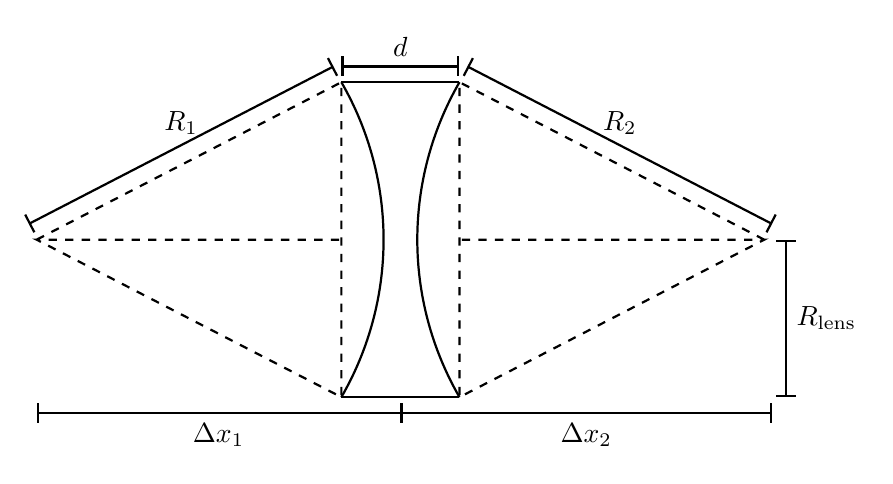
\begin{tikzpicture}
        % Note (0, 2) is where tikz starts drawing the arc
        \draw[thick] (0, 2) arc (150:210:4);
        \draw[thick] (-1.5, 2) arc (30:-30:4);
        \draw[thick] (0, 2) -- (-1.5, 2);
        \draw[thick] (0, -2) -- (-1.5, -2);
        
        \draw[thick, |-|] (-1.5, 2.2) -- (0.0, 2.2) node[pos=0.5, above] {$d$};
        
        % Dashed lines on left & labels
        \draw[thick, dashed]  (-5.37,0) -- (-1.5, 2) -- (-1.5, -2) -- (-5.37,0) -- (-1.5, 0);
        
        \draw[thick, -|] (-0.75, -2.2) -- (-5.37, -2.2) node[pos=0.5, below] {$\Delta x_1$};
        \draw[thick, |-|] (-1.6, 2.2) -- (-5.47, 0.2) node[pos=0.5, above] {$R_1$};
        
        % Dashed lines on right & labels
        \draw[thick, dashed]  (3.87,0) -- (0, 2) -- (0, -2) -- (3.87,0) -- (0, 0);
        
        \draw[thick, |-|] (-0.75, -2.2) -- (3.97, -2.2) node[pos=0.5, below] {$\Delta x_2$};
        \draw[thick, |-|] (0.1, 2.2) -- (3.97, 0.2) node[pos=0.5, above] {$R_2$};
        
        % R_lens on right
        \draw[thick, |-|] (4.15, 0.0) -- (4.15, -2.0) node[pos=0.5, right] {$R_\mathrm{lens}$};
    \end{tikzpicture}

    \caption{Left: Parameters used to describe a lens, in this case a biconcave. $R_1$ and $R_2$ are the radii of curvature on the left and right sides respectively. $\Delta x_1$ and $\Delta x_2$ give the horizontal offset between the centre of the lens and each arc respectively. $R_\mathrm{lens}$ give the radius of the lens and $d$ its thickness.}
    \label{fig:convex lens}
\end{figure}


\section{Calling from Python}
\label{sec:calling from python}
To call from Python we wrap the C++ using Cython. We wrap each C++ class to produce a similarly named class as that in C++ but roughly with ``Py" at the front. Class equivalents are detailed in Tab.~\ref{tab:C++ to Cython mappings}. Similarly we also produce a tracing function that takes in Python components and traces them in C++ named \texttt{PyTrace}.

\begin{table}[h!]
\centering
    \begin{tabular}{ |c|c| } 
         \hline
         C++ & Cython \\ 
         \hline
         \texttt{Component} & \texttt{\_PyComponent} \\ 
         \texttt{Complex\_Component} & \texttt{PyComplex\_Complex} \\ 
         \texttt{Plane} & \texttt{\_PyPlane} \\ 
         \texttt{Spherical} & \texttt{\_PySpherical} \\ 
         \texttt{Mirror\_Plane} & \texttt{PyMirror\_Plane} \\ 
         \texttt{Refract\_Plane} & \texttt{PyRefract\_Plane} \\ 
         \texttt{Mirror\_Sph} & \texttt{PyMirror\_Sph} \\ 
         \texttt{Refract\_Sph} & \texttt{PyRefract\_Sph} \\ 
         \texttt{Screen\_Plane} & \texttt{PyScreen\_Plane} \\
         \texttt{Ray} & \texttt{PyRay} \\ 
         \hline
         
    \end{tabular}
    \caption{C++ classes and their equivalent Cython versions.}
    \label{tab:C++ to Cython mappings}
\end{table}

Properties such as the start and end points of planes are exposed as properties. In most cases points are returned as a NumPy view. As such they may be edited element wise if the view is writable. The notable exception to this is \texttt{PyRay.pos} which returns a copy due to the way \texttt{Ray.pos} is stored in C++.

Furthermore, we have some additional classes. \texttt{PyCC\_Wrap} is intended to allow easy creation of complex components from Python by simply inheriting from \texttt{PyCC\_Wrap} and passing the Cython components needed to describe the component to the \texttt{PyCC\_Wrap} initialiser. For example, a triangular prism defined through the positions of its vertices and interior/exterior refractive indices can be created using:
\begin{lstlisting}[language=Python]
class Prism(PyCC_Wrap):
    def __init__(self, a, b, c, n_in, n_out=1.0):
        comps = [
                PyRefract_Plane(a, b, n_out, n_in),
                PyRefract_Plane(b, c, n_out, n_in),
                PyRefract_Plane(c, a, n_out, n_in)
            ]
            
        # Must remember to call super __init__()
        super().__init__(comps)  
\end{lstlisting}
Like other components, \texttt{PyCC\_Wrap} provides a \texttt{Plot()} method useful for plotting the component.

In addition to these classes, we also provide \texttt{PyLens} and \texttt{PyBiConvexLens} to model a generic lens and a bi-convex lens.

% Bibliography
\bibliographystyle{ieeetr}
\bibliography{bibo}

\end{document}
